% arara: xelatex
% arara: xelatex
% arara: xelatex

% options:
% thesis=B bachelor's thesis
% thesis=M master's thesis
% czech thesis in Czech language
% english thesis in English language
% hidelinks remove colour boxes around hyperlinks

\documentclass[thesis=M,english]{FITthesis}[2019/12/23]

\usepackage[utf8]{inputenc} % LaTeX source encoded as UTF-8

\usepackage{graphicx} %graphics files inclusion
\usepackage{amsmath} %advanced maths
\usepackage{amssymb} %additional math symbols 
\usepackage{mathtools,amscd}

\usepackage{dirtree} %directory tree visualisation
\usepackage{listings}
\usepackage{pdfpages}
\usepackage{float}
\usepackage{svg}

\usepackage{mmacells}
\mmaSet{leftmargin=2em}

% % list of acronyms
% \usepackage[acronym,nonumberlist,toc,numberedsection=autolabel]{glossaries}
% \iflanguage{czech}{\renewcommand*{\acronymname}{Seznam pou{\v z}it{\' y}ch zkratek}}{}
% \makeglossaries

% % % % % % % % % % % % % % % % % % % % % % % % % % % % % % 
% EDIT THIS
% % % % % % % % % % % % % % % % % % % % % % % % % % % % % % 

\department{Department of Information Security}
\title{Multivariate cryptography}
\authorGN{Jan} %author's given name/names
\authorFN{Rahm} %author's surname
\author{Jan Rahm} %author's name without academic degrees
\authorWithDegrees{Bc. Jan Rahm} %author's name with academic degrees
\supervisor{Ing. Jiří Buček, Ph.D.}
\acknowledgements{I would like to thank Ing. Jiří Buček, Ph.D. for the willingness, consultation and valuable advice he gave me.}
\abstractEN{The diploma thesis deals with selected algorithms of multivariate cryptography, especially Unbalanced Oil \& Vintage and Rainbow. The aim of this work is implementation of algorithms in Wolfram Mathematica, investigation of existing solutions and their implementation on ESP32 microcontroller. The algorithms are tested and measured against the RSA and ECDSA algorithms.}
\abstractCS{Diplomová práce se zabývá vybranými algoritmy multivariační kryptografie, zejména Unbalanced Oil \& Vintage a Rainbow. Cílem práce je implementace algoritmů ve Wolfram Mathematica, prozkoumání již existujících řešeních a jejich implementace na mikrokontroleru ESP32. Algoritmy jsou otestovány a změřeny vůči algoritmům RSA a ECDSA.}
\placeForDeclarationOfAuthenticity{Prague}
\keywordsCS{Multivariační kryptografie, Unbalanced Oil \& Vintage, Rainbow, Wolfram Mathematica, ESP32}
\keywordsEN{Multivariate cryptography, Unbalanced Oil \& Vintage, Rainbow, Wolfram Mathematica, ESP32}
\declarationOfAuthenticityOption{1} %select as appropriate, according to the desired license (integer 1-6)
\website{https://github.com/rahmjan/Diploma_Thesis} %optional thesis URL

\begin{document}

% \newacronym{CVUT}{{\v C}VUT}{{\v C}esk{\' e} vysok{\' e} u{\v c}en{\' i} technick{\' e} v Praze}
% \newacronym{FIT}{FIT}{Fakulta informa{\v c}n{\' i}ch technologi{\' i}}

%%%%%%%%%%%%%%%%%%%%%%%%%%%%%%%%%%%%%%%%%%%%
%%%%%%%%%%%%%%%%%%%%%%%%%%%%%%%%%%%%%%%%%%%%
\setsecnumdepth{part}
\chapter{Introduction}
Cryptography is one of the most needed part of modern informatics because almost everyone has something they wish to stay private. But today we can see uprise of the quantum computers which are able to decipher the conventional algorithms for cryptology. That is why a new category of post-quantum cryptography was created and one of its candidates is multivariate cryptography.

The objective of this work is to describe principles of multivariate cryptography for educational purpose with creation of simple example in Wolfram Mathematica. The focus is on Unbalanced Oil \& Vintage and Rainbow algorithms with examination of reference implementation. Further focusing on possible implementation on ESP32 and possible use in IoT.

The final part belongs to comparison with conventional algorithms which are RSA and ECDSA.

%%%%%%%%%%%%%%%%%%%%%%%%%%%%%%%%%%%%%%%%%%%%
%%%%%%%%%%%%%%%%%%%%%%%%%%%%%%%%%%%%%%%%%%%%
\setsecnumdepth{all}
\chapter{Basic terms and definitions}
The chapter describes concepts and algorithms used in the thesis.

\section{Basic terms}
\subsection{Polynomial}
Polynomial $p$ is function to which applies
\[
	p(x) = \sum\limits_{i=0}^n {\alpha_ix^i} = \alpha_0 + \alpha_1x + \alpha_2x^2 + ... + \alpha_nx^n,
\]
where $n \in N_0$ and $\alpha_0, \alpha_1, ..., \alpha_n \in R$. Values $\alpha_0, \alpha_1, ..., \alpha_n$ we calls polynomial coefficients of $p$.  

\subsection{Degree of a polynomial}
The degree of a polynomial is the highest index $i \in N_0$ to which applies that coefficient $\alpha_i \ne 0$. If all coefficients are zero, then the degree of the polynomial is -1.

\subsection{Post-quantum cryptography}
It refers to algorithms that are thought to be secure against an attack by a quantum computer.

But today it is not true for the most used cryptographic algorithms, which are based on mathematical problems of integer factorization, discrete logarithm or elliptic-curve discrete logarithm. These problems can be solved by Shor's algorithm on quantum computer.

\subsection{Finite field}
A finite field is a finite set which is a field. This means that multiplication, addition, subtraction and division (excluding division by zero) are defined and satisfy the rules of arithmetic known as the field axioms.

The simplest examples of finite fields are the fields of prime order: $\mathbb {F}_{p}$ may be constructed as the integers modulo p.

\subsection{Translation}
In Euclidean geometry, a translation is a geometric transformation that moves every point of a figure or a space by the same distance in a given direction.

\subsection{Linear map}
In mathematics, a linear map is a mapping $V \rightarrow W$ between two modules (for example, two vector spaces) that preserves the operations of addition and scalar multiplication.

\subsection{Affine map}
An affine map is the composition of two functions: a translation and a linear map. Ordinary vector algebra uses matrix multiplication to represent linear maps, and vector addition to represent translations. Formally, in the finite-dimensional case, if the linear map is represented as a multiplication by a matrix $A$ and the translation as the addition of a vector $\vec {b}$, an affine map $f$ acting on a vector ${\vec {x}}$ can be represented as:
\[
{\vec {y}}=f({\vec {x}})=A{\vec {x}}+{\vec {b}}
\]

\subsection{Wolfram Mathematica}
\subsection{IoT}
\subsection{ESP32}
\subsection{RSA}
\subsection{ECDSA}

%%%%%%%%%%%%%%%%%%%%%%%%%%%%%%%%%%%%%%%%%%%%
\section{Multivariate cryptography}
\subsection{Definition}
"Multivariate cryptography (MC) is the generic term for asymmetric cryptographic primitives based on multivariate polynomials over a finite field $\mathbb{F}$."\cite{L-WIKI1}

It means it is system of nonlinear polynomial equations with coefficients over a finite filed $\mathbb{F} = \mathbb{F}_q$ with $q$ elements:
\[
	p^{(1)}(x_1,\ldots,x_n) = \sum\limits_{i=1}^{n} {\sum\limits_{j=1}^{n} {p_{ij}^{(1)} \cdot x_ix_j}} + \sum\limits_{i=1}^{n} {p_{i}^{(1)} \cdot x_i} + p_0^{(1)}
\]
\[
	p^{(2)}(x_1,\ldots,x_n) = \sum\limits_{i=1}^{n} {\sum\limits_{j=1}^{n} {p_{ij}^{(2)} \cdot x_ix_j}} + \sum\limits_{i=1}^{n} {p_{i}^{(2)} \cdot x_i} + p_0^{(2)}
\]
\[
	\vdots
\]
\[
	p^{(m)}(x_1,\ldots,x_n) = \sum\limits_{i=1}^{n} {\sum\limits_{j=1}^{n} {p_{ij}^{(m)} \cdot x_ix_j}} + \sum\limits_{i=1}^{n} {p_{i}^{(m)} \cdot x_i} + p_0^{(m)}
\]
 
If the polynomials are of degree two, they are called multivariate quadratics (MQ). Solving systems of multivariate polynomial equations is proven to be NP hard, so called MQ Problem. That is the reason why MC is often considered to be good candidate for post-quantum cryptography.

MC is very fast and requires only moderate computational resources, which makes it attractive for applications in low-cost devices.

\subsection{MQ Problem}
Given $m$ quadratic polynomials $p^{(1)}(x),\ldots,p^{(m)}(x)$ in the $n$ variables $x_1,\ldots,x_n$, find a vector $\bar{x} = (\bar{x}_1,\ldots,\bar{x}_n)$ such that $p^{(1)}(\bar{x}) = \ldots = p^{(m)}(\bar{x}) = 0$.

\subsection{Public key}
The public key of MC is system of MC polynomials. To build this system based on MQ Problem, it needs an easily invertible quadratic map $\mathcal{F}: \mathbb{F}^n \rightarrow \mathbb{F}^m$, so called \textit{central map}. Because it is easily invertible, it needs to be hidden in public key by invertible affine maps: $\mathcal{S}: \mathbb{F}^m \rightarrow \mathbb{F}^m$ and $\mathcal{T}: \mathbb{F}^n \rightarrow \mathbb{F}^n$.

The public key of this system is composed map:
\[
	\mathcal{P} = \mathcal{S} \circ \mathcal{F} \circ \mathcal{T} : \mathbb{F}^n \rightarrow \mathbb{F}^m
\]
and the private key consists of the tree maps $\mathcal{S}$, $\mathcal{F}$ and $\mathcal{T}$, also known as \textit{trapdoor}.

Public key should be hard to invert without the knowledge of the \textit{trapdoor}.

\begin{figure}[h]
\begin{equation*}
  \begin{CD}
     z \in \mathbb{F}^n @>  \mathcal{P} >> w \in \mathbb{F}^m \\
    @V\mathcal{T}VV  @A\mathcal{S}AA \\
  y \in \mathbb{F}^n @> \mathcal{F} >> x \in \mathbb{F}^m
  \end{CD}
\end{equation*}
\caption{Workflow of multivariate public key cryptosystems}
\end{figure}
\smallskip

\subsection{Encryption}
To get a ciphertext $w$, message $z \in \mathbb{F}^n$ can by easily encrypted by evaluation of the public key $\mathcal{P}$:
\[
	w = \mathcal{P}(z) \in \mathbb{F}^m
\]
For decryption of ciphertext, it needs to be evaluated by private key in tree steps: 
\[
	x = \mathcal{S}^{-1}(w) \in \mathbb{F}^m, \, y = \mathcal{F}^{-1}(x) \in \mathbb{F}^n, \, z = \mathcal{T}^{-1}(y) \in \mathbb{F}^n
\]
There is a condition that requires to be $m \geq n$, this way the public key $\mathcal{P}$ will be injective and decryption will output a unique plaintext.

\subsection{Signature}
To generate a signature for a message $m$, it needs to use a hash function:
\[
	\mathcal{H}: \{0,1\}^{*} \rightarrow \mathbb{F}^m
\]
to compute the hash value:
\[
	w = \mathcal{H}(m) \in \mathbb{F}^m
\]
After this step it can be evaluated by:
\[
	x = \mathcal{S}^{-1}(w) \in \mathbb{F}^m, \, y = \mathcal{F}^{-1}(x) \in \mathbb{F}^n, \, z = \mathcal{T}^{-1}(y) \in \mathbb{F}^n
\]
where $z$ is the signature of message $m$. As can be seen, it is similar to description of ciphertext.

The verification of signature $z$ is done by computing the hash value:
\[
	w = \mathcal{H}(m) \in \mathbb{F}^m
\]
and by evaluation of public key $\mathcal{P}$:
\[
	w' = \mathcal{P}(z) \in \mathbb{F}^m
\]
If $w' = w$ is true, the signature is valid, otherwise not.

There is also condition that requires to be $m \leq n$, this way the public key $\mathcal{P}$ will be surjective and private key can sign any message.

%%%%%%%%%%%%%%%%%%%%%%%%%%%%%%%%%%%%%%%%%%%%
\section{UOV}
The Unbalanced Oil and Vinegar's name comes from the fact that the variables of the polynomials are grouped into two groups: the vinegar and the oil. These two groups are mixed in the polynomials and the unbalanced attribute refers to the ratio of the variables, where is always more vinegar than oil variables. The signature scheme was proposed by Kipnis and Patarin in 1999.

\subsection{Definition}
Let $\mathbb{F}$ be a finite field, $v,o \in \mathbb{N}$ and $n=v+o$, $V=\{1, \ldots, v\}$, $O=\{v+1, \ldots, n\}$. The variables $x_1, \ldots, x_v$ are Vinegar variables and $x_{v+1}, \ldots, x_n$ are Oil variables. If $v=o$ the scheme is called balanced Oil \& Vinegar (OV), for $v>o$ it is UOV.

\bigskip
\noindent
The \textit{central map} $\mathcal{F}:\mathbb{F}^n \rightarrow \mathbb{F}^o$ consist of $o$ quadratic polynomials $f^{(1)}, \ldots, f^{(o)}$:
\[
	f^{(k)} = \sum\limits_{i=1}^{v} {\sum\limits_{j=1}^{v} {\alpha_{ij}^{(k)} \cdot x_ix_j}} +  \sum\limits_{i=1}^{v} {\sum\limits_{j=v+1}^{n} {\beta_{ij}^{(k)} \cdot x_ix_j}}+ \sum\limits_{i=1}^{n} {\gamma_{i}^{(k)} \cdot x_i} + \delta^{(k)}
\]
where $\alpha_{ij}^{(k)}$, $\beta_{ij}^{(k)}$, $\gamma_{i}^{(k)}$, $\delta^{(k)} \in \mathbb{F}$ and $1 \leq k \leq o$.

\bigskip
\noindent
To hide $\mathcal{F}$ in the public key, it is combined with one invertible affine map $\mathcal{T}: \mathbb{F}^n \rightarrow \mathbb{F}^n$. The public key of the scheme is in the form:
\[
	\mathcal{P} = \mathcal{F} \circ \mathcal{T} : \mathbb{F}^n \rightarrow \mathbb{F}^o
\]
and the private key consist of $\mathcal{F}$ and $\mathcal{T}$. The second affine map $\mathcal{S}$ is not needed for the security of UOV.

\subsection{Security}
For the security of UOV is required $v \geq 2o$ because of the attack of Kipnis and Shamir on balanced OV.\cite{L-KS98} Besides of that, the UOV scheme resisted (for suitable parameter sets) cryptanalysis for over 20 years. Now it is one of the oldest and best studied cryptosystems and is therefore believed to be of high security.

The UOV scheme is very simple, has small signatures and is fast. The main disadvantage is its public keys which are quite large.

%%%%%%%%%%%%%%%%%%%%%%%%%%%%%%%%%%%%%%%%%%%%
\section{Rainbow}
The Rainbow is a multi layer version of UOV. The layers are not independent from each other but there is a hierarchy which uses the results from the layer above to compute additional variables. The name comes from the link to the layers of a rainbow and the scheme was introduced by Ding and Schmid in 2005.

The main advantage compared to UOV should be in better performance, smaller key sizes and smaller signatures.

\subsection{Definition}
Let $\mathbb{F}$ be a finite field, $0<v_1<v_2<\ldots<v_{u+1} = n$ be a sequence of integers and $V_i=\{1, \ldots, v_i\}$, $O_i=\{v_i+1, \ldots, v_{i+1}\}$ and $o_i = v_{i+1} - v_i \,\, (i=1,\ldots,u)$ where $o_i$ is number of oil variables and $u$ is number of UOV instances.

\bigskip
\noindent
The \textit{central map} $\mathcal{F}:\mathbb{F}^n \rightarrow \mathbb{F}^m$ consist of $m = n - v_1$ quadratic polynomials $f^{(v_1+1)}, \ldots, f^{(n)}$:
\[
	f^{(k)} = \sum\limits_{i,j \in V_l}{\alpha_{ij}^{(k)} \cdot x_ix_j} +  \sum\limits_{i \in V_l,j \in O_l}{\beta_{ij}^{(k)} \cdot x_ix_j}+ \sum\limits_{i \in V_l \cup O_l}{\gamma_{i}^{(k)} \cdot x_i} + \delta^{(k)}
\]
where $l \in \{1, \ldots, u\}$ is the only integer such that $k \in O_l$ and $\alpha_{ij}^{(k)}$, $\beta_{ij}^{(k)}$, $\gamma_{i}^{(k)}$, $\delta^{(k)} \in \mathbb{F}$.

\bigskip
\noindent
To hide $\mathcal{F}$ in the public key, it is combined with two invertible affine maps $\mathcal{T}: \mathbb{F}^n \rightarrow \mathbb{F}^n$ and $\mathcal{S}: \mathbb{F}^m \rightarrow \mathbb{F}^m$. The public key of the scheme is in the form:
\[
	\mathcal{P} = \mathcal{S} \circ \mathcal{F} \circ \mathcal{T} : \mathbb{F}^n \rightarrow \mathbb{F}^m
\]
and the private key consist of $\mathcal{S}$, $\mathcal{F}$ and $\mathcal{T}$.

%%%%%%%%%%%%%%%%%%%%%%%%%%%%%%%%%%%%%%%%%%%%
%%%%%%%%%%%%%%%%%%%%%%%%%%%%%%%%%%%%%%%%%%%%
\chapter{Realization}
Add description...

\section{Wolfram Mathematica}
This section describes examples in Wolfram Mathematica and step by step description of algorithms.

\subsection{UOV}
Here is description of signature scheme of UOV. This example of UOV is in fact example of balanced OV because it simplify the explanation of the algorithm.

\bigskip
\noindent
First set up the parameters of the example: 
Let $\mathbb{F} = GF(7)$, $o=v=3$. The central map $\mathcal{F} = (f^{(1)}, f^{(2)}, f^{(3)})$ is given by:
\begin{mmaCell}[addtoindex=2,moredefined={mod, F1, F2, F3},morepattern={x1_, x2_, x3_, x4_, x5_, x6_, x1, x2, x3, x4, x5, x6}]{Input}
  mod=7;
  F1[x1_,x2_,x3_,x4_,x5_,x6_]:=
4x1^2+4x1*x3+5x1*x4+6x1*x5+x1*x6+6x1+4x2^2+x2*x3+6x2*x4
+6x2*x5+5x2*x6+5x2+5x3^2+3x3*x4+5x3*x5+2x3*x6+5x3+6x4+3x5;
  F2[x1_,x2_,x3_,x4_,x5_,x6_]:=
3x1*x3+4x1*x4+3x1*x5+4x1*x6+3x1+6x2^2+x2*x3+4x2*x4+4x2*x5
+5x2*x6+6x2+6x3^2+4x3*x4+2x3*x5+x3*x6+3x3+x4+x6+1;
  F3[x1_,x2_,x3_,x4_,x5_,x6_]:=
6x1^2+6x1*x3+4x1*x5+2x1*x6+2x2^2+5x2*x3+6x2*x4+5x2*x5+
5x2*x6+6x2+3x3^2+5x3*x4+6x3*x5+x3*x6+3x3+4x4+6x5+5;
\end{mmaCell}
It will set up the value of $mod$ to 7 and initialize functions of the central map. Next is setting up of the affine map $\mathcal{T}$ with matrix $A$ and vector $b$. These two parts will be later used separately in the example. 
\begin{figure}[h]
	\begin{minipage}{0.42\textwidth}
		\centering
		\begin{mmaCell}[addtoindex=3,moredefined={A}]{Input}
  A=(6 5 5 5 5 4
     6 6 4 5 0 6
     2 5 2 1 5 0
     1 1 6 2 2 3
     3 6 2 2 3 0
     0 5 4 6 1 5);
		\end{mmaCell}
	\end{minipage}
	\begin{minipage}{0.28\textwidth}
		\centering
		\begin{mmaCell}[moredefined={b}]{Input}
  b=(1
     2
     4
     1
     3
     2);
		\end{mmaCell}
	\end{minipage}
	\begin{minipage}{0.2\textwidth}
		\centering
		\begin{mmaCell}[moredefined={T, A, b}]{Input}
  T=A.(x1
       x2
       x3
       x4
       x5
       x6)+b; 
		\end{mmaCell}
	\end{minipage}
\end{figure}

\noindent
This block computes public key $\mathcal{P}$ by putting values of $\mathcal{T}$ inside of $\mathcal{F}$, it also simplify the expression of $p1,p2,p3$ and finally applies modulo on whole polynomial:
\begin{mmaCell}[moredefined={p1, F1, T, p2, F2, p3, F3, P1, mod, P2, P3},morepattern={x1_, x2_, x3_, x4_, x5_, x6_}]{Input}
  p1 = F1 @@ T[[All]];
  p2 = F2 @@ T[[All]];
  p3 = F3 @@ T[[All]];
  P1[x1_,x2_,x3_,x4_,x5_,x6_] = PolynomialMod[Simplify[p1],mod]
  P2[x1_,x2_,x3_,x4_,x5_,x6_] = PolynomialMod[Simplify[p2],mod]
  P3[x1_,x2_,x3_,x4_,x5_,x6_] = PolynomialMod[Simplify[p3],mod]
\end{mmaCell}

\noindent
The results of $\mathcal{P} = \mathcal{F} \circ \mathcal{T}$ are:
\begin{mmaCell}[addtoindex=3]{Output}
  \{6+x1+5x2+4x1x2+2\mmaSup{x2}{2}+3x3+x1x3+x2x3+\mmaSup{x3}{2}+6x4+2x1x4+5x2x4+2x3x4
+3\mmaSup{x4}{2}+5x5+3x1x5+6x2x5+4x3x5+3x4x5+4\mmaSup{x5}{2}+4x6+x2x6+3x3x6+2x4x6\}
\end{mmaCell}
\begin{mmaCell}{Output}
  \{5+6\mmaSup{x1}{2}+5x2+4x1x2+5\mmaSup{x2}{2}+4x3+5x1x3+3x2x3+2\mmaSup{x3}{2}+2x4+2x1x4+4x2x4
+2x3x4+5\mmaSup{x4}{2}+3x5+5x1x5+5x2x5+2x3x5+6\mmaSup{x5}{2}+5x2x6+6x4x6+2x5x6+6\mmaSup{x6}{2}\}
\end{mmaCell}
\begin{mmaCell}{Output}
  \{5+5x1+4\mmaSup{x1}{2}+5x2+3x1x2+5\mmaSup{x2}{2}+2x3+2x1x3+x2x3+2\mmaSup{x3}{2}+6x4+3x2x4+2\mmaSup{x4}{2}
+x5+3x1x5+6x2x5+4x3x5+2\mmaSup{x5}{2}+2x6+x1x6+3x2x6+4x3x6+6x4x6+5x5x6+4\mmaSup{x6}{2}\}
\end{mmaCell}
From this place on it will only focus on computation of signature $z$ for message $w$. Be aware that in this example is not used hash function for the message because for the example purpose it is not needed.
\begin{mmaCell}[moredefined={w, y1, y2, y3}]{Input}
  w  = \{\{3\},\{6\},\{4\}\};
  y1 = 1;
  y2 = 0;
  y3 = 6;
\end{mmaCell}
It sets the message to value $w = (3,6,4)$ and also it set values for $y = (y1,y2,y3)$. These values for $y$ are randomly chosen.
\begin{mmaCell}[addtoindex=3,moredefined={f1, F1, y1, y2, y3, mod, f2, F2, f3, F3}]{Input}
  f1 = PolynomialMod[F1[y1,y2,y3,y4,y5,y6],mod]
  f2 = PolynomialMod[F2[y1,y2,y3,y4,y5,y6],mod]
  f3 = PolynomialMod[F3[y1,y2,y3,y4,y5,y6],mod]
\end{mmaCell}
Here are the results after minimalizing and use of modulo:
\begin{mmaCell}{Output}
  f1 = 6+y4+4y5+6y6
  f2 = 4+y4+y5+4y6
  f3 = 5+6y4+4y5+y6
\end{mmaCell}
Next two steps solve linear system $f^{(1)} = w_1 = 3, f^{(2)} = w_2 = 6, f^{(3)} = w_3 = 4$, it can also use for the solution the Gaussian elimination:
\begin{mmaCell}[moredefined={res, f1, w, f2, f3, mod}]{Input}
  res = Solve[\{f1==w[[1]], f2==w[[2]], f3==w[[3]]\},Modulus \(\pmb{\to}\) mod];
\end{mmaCell}
\begin{mmaCell}[moredefined={y, y1, y2, y3, res}]{Input}
  y = \{y1,y2,y3,y4,y5,y6\} /. res 
\end{mmaCell}
\begin{mmaCell}{Output}
  \{\{1,0,6,6,3,0\}\}
\end{mmaCell}
It will obtain results for $(y4,y5,y6) = (6,3,0)$. After combination it is $y = (1,0,6,6,3,0)$, so called \textit{pre-image} of $w$: $y =  \mathcal{F}^{-1}(w)$. If the solution for linear system do not exist, choose different values for $(y1,y2,y3)$ and repeat steps before.

\bigskip
\noindent
Finally use $\mathcal{T}^{-1}$ to compute signature $z$. For that is needed inversion of matrix $A$.
\begin{figure}[h]
	\begin{minipage}{0.59\textwidth}
		\centering
\begin{mmaCell}[moredefined={A, mod}]{Input}
  \mmaSub{A}{-1} = Inverse[A, Modulus\(\pmb{\to}\)mod]
\end{mmaCell}
	\end{minipage}
	\begin{minipage}{0.28\textwidth}
		\centering
		\begin{equation*}
A_{-1} = 
\begin{pmatrix}
2 & 4 & 6 & 2 & 0 & 5 \\
1 & 3 & 3 & 1 & 6 & 2 \\
4 & 6 & 6 & 4 & 5 & 4 \\
2 & 0 & 3 & 4 & 2 & 3 \\
6 & 0 & 3 & 0 & 0 & 5 \\
2 & 2 & 2 & 5 & 3 & 3
\end{pmatrix}
\end{equation*}
	\end{minipage}
\end{figure}
\begin{mmaCell}[moredefined={z, A, y, b, mod}]{Input}
  z = Mod[\mmaSub{A}{-1}.(Transpose[y]-b),mod] 
\end{mmaCell}
\begin{mmaCell}{Output}
  \{\{4\},\{1\},\{5\},\{6\},\{3\},\{5\}\}
\end{mmaCell}
The value of the signature $z = (4,1,5,6,3,5)$.

\bigskip
\noindent
Last part is check if two hashes (in this example two messages $w$) are the same.
\begin{mmaCell}[moredefined={w2, w, P1, z, P2, P3, mod}]{Input}
  w2=w;
  w2=\{P1 @@ z[[All,1]],P2 @@ z[[All,1]],P3 @@ z[[All,1]]\};
  (* True? *)
  Mod[w2,mod]==w
\end{mmaCell}
\begin{mmaCell}[addtoindex=2]{Output}
  True
\end{mmaCell}

The file with implementation can by find under name "UOV.nb".

\subsection{Rainbow}
The description of signature scheme of Rainbow is very similar to the description of OV.

\bigskip
\noindent
First set up the parameters of the example: 
Let $\mathbb{F} = GF(7)$, $v1=o1=o2=2$. The central map $\mathcal{F} = (f^{(3)}, f^{(4)}, f^{(5)}, f^{(6)})$ is given by:
\begin{mmaCell}[addtoindex=2,moredefined={mod, F3, F4, F5, F6},morepattern={x1_, x2_, x3_, x4_, x5_, x6_, x1, x2, x3, x4, x5, x6}]{Input}
  mod=7;
  F3[x1_,x2_,x3_,x4_,x5_,x6_]:= 
x1^2+3x1*x2+5x1*x3+6x1*x4+2x2^2+6x2*x3+4x2*x4+2x2+6x3+2x4+5;
  F4[x1_,x2_,x3_,x4_,x5_,x6_]:= 
2x1^2+x1*x2+x1*x3+3x1*x4+4x1+x2^2+x2*x3+4x2*x4+6x2+x4;
  F5[x1_,x2_,x3_,x4_,x5_,x6_]:= 
2x1^2+3x1*x2+3x1*x3+3x1*x4+x1*x5+3x1*x6+6x1+4x2^2+x2*x3+
4x2*x4+x2*x5+3x2*x6+3x2+3x3*x4+x3*x5+2x3*x6+2x3+3x4*x5+x5+6x6;
  F6[x1_,x2_,x3_,x4_,x5_,x6_]:= 
2x1^2+5x1*x2+x1*x3+5x1*x4+5x1*x6+6x1+5x2^2+3x2*x3+5x2*x5+4x2*x6
+x2+3x3^2+5x3*x4+4x3*x5+2x3*x6+4x3+x4^2+6x4*x5+3x4*x6+4x4+4x5+x6+2;
\end{mmaCell}
Next is setting up of the affine map $\mathcal{T}$ with matrix $A$ and vector $b$ which are the same as in OV example. But with addition of affine map $\mathcal{S}$ with matrix $A2$ and vector $b2$.
\begin{figure}[h]
	\begin{minipage}{0.39\textwidth}
		\centering
		\begin{mmaCell}[addtoindex=3,moredefined={A2}]{Input}
  A2=(6 5 5 5
      6 6 4 5
      2 5 2 1
      1 1 6 2);
		\end{mmaCell}
	\end{minipage}
	\begin{minipage}{0.3\textwidth}
		\centering
		\begin{mmaCell}[moredefined={b2}]{Input}
  b2=(1
      2
      4
      1);
		\end{mmaCell}
	\end{minipage}
	\begin{minipage}{0.2\textwidth}
		\centering
		\begin{mmaCell}[moredefined={S, A2, b2}]{Input}
  S=A2.(x1
        x2
        x3
        x4)+b2; 
		\end{mmaCell}
	\end{minipage}
\end{figure}

\noindent
This block computes public key $\mathcal{P}$ by putting values of $\mathcal{T}$ inside of $\mathcal{F}$ and after it makes from matrix S functions which are used for final step of computation of $\mathcal{P}$, it also simplify the expression of $pp3,pp4,pp5,pp6$ and finally applies modulo on whole polynomial:
\begin{mmaCell}[moredefined={p3, p4, p5, p6, S3, S4, S5, S6, mod, P3, P4, P5, P6, pp3,pp4,pp5,pp6, F3, F4, F5,F6, T, S},morepattern={x1_, x2_, x3_, x4_, x5_, x6_}]{Input}
p3 = F3 @@ T[[All]];
p4 = F4 @@ T[[All]];
p5 = F5 @@ T[[All]];
p6 = F6 @@ T[[All]];
S3[x1_,x2_,x3_,x4_] = S[[1]];
S4[x1_,x2_,x3_,x4_] = S[[2]];
S5[x1_,x2_,x3_,x4_] = S[[3]];
S6[x1_,x2_,x3_,x4_] = S[[4]];
pp3 = S3[p3,p4,p5,p6][[1]];
pp4 = S4[p3,p4,p5,p6][[1]];
pp5 = S5[p3,p4,p5,p6][[1]];
pp6 = S6[p3,p4,p5,p6][[1]];
P3[x1_,x2_,x3_,x4_,x5_,x6_] = PolynomialMod[Simplify[pp3],mod];
P4[x1_,x2_,x3_,x4_,x5_,x6_] = PolynomialMod[Simplify[pp4],mod];
P5[x1_,x2_,x3_,x4_,x5_,x6_] = PolynomialMod[Simplify[pp5],mod];
P6[x1_,x2_,x3_,x4_,x5_,x6_] = PolynomialMod[Simplify[pp6],mod];
\end{mmaCell}

\noindent
Computation $x$ from message $w$: $x = \mathcal{T}^{-1}(w)$ :
\begin{mmaCell}[moredefined={w, A2, b2, S, x, mod}]{Input}
w = \{\{2\},\{2\},\{3\},\{4\}\};
\mmaSub{A2}{-1} = Inverse[A2, Modulus\(\pmb{\to}\)mod]
x = Mod[\mmaSub{A2}{-1}.(w - b2),mod]
\end{mmaCell}
\begin{mmaCell}{Output}
  \{\{6\},\{0\},\{1\},\{6\}\}
\end{mmaCell}

\noindent
The result is $x = (6,0,1,6)$.

\bigskip
\noindent
Next is computation of \textit{pre-image} for $x$ and also the place where is the biggest difference from OV scheme, let's start with the first step where is set up of random values for $y1, y2$ and makes their substitution in the polynomials:
\begin{mmaCell}[moredefined={y1, y2, f3, f4, f5, f6, mod, F3, F4, F5, F6}]{Input}
y1 = 0;
y2 = 1;
f3 = PolynomialMod[F3[y1,y2,x3,x4,x5,x6],mod];
f4 = PolynomialMod[F4[y1,y2,x3,x4,x5,x6],mod];
f5 = PolynomialMod[F5[y1,y2,x3,x4,x5,x6],mod];
f6 = PolynomialMod[F6[y1,y2,x3,x4,x5,x6],mod];
\end{mmaCell}
\begin{mmaCell}{Output}
  f3 = 2+5x3+6x4
  f4 = x3+5x4
  f5 = 3x3+4x4+3x3x4+2x5+x3x5+3x4x5+2x6+2x3x6
  f6 = 1+3x3^2+4x4+5x3x4+x4^2+2x5+4x3x5+6x4x5+5x6+2x3x6+3x4x6
\end{mmaCell}
For the second step it is visible from the result that $f^{(3)}$ and $f^{(4)}$ are two equations with two unknown values.
\begin{mmaCell}[moredefined={res1, f3, f4, x, mod}]{Input}
  res1 = Solve[\{f3==x[[1]],f4==x[[2]]\},Modulus \(\pmb{\to}\) mod];
\end{mmaCell}
It solves and with these two values $(x3, x4)$, it is possible to continue the substitution and to compute the final linear system (repeat the first and second steps):
\begin{mmaCell}[moredefined={res1, y1, y2, mod, F5, F6, f5, f6}]{Input}
  f5 = PolynomialMod[F5[y1,y2,x3,x4,x5,x6]/.res1,mod];
  f6 = PolynomialMod[F6[y1,y2,x3,x4,x5,x6]/.res1,mod];
\end{mmaCell}
\begin{mmaCell}{Output}
  f5 = 2+5x5+3x6
  f6 = 3+2x5+5x6
\end{mmaCell}
\begin{mmaCell}[moredefined={res2, f5, f6, x, mod}]{Input}
  res2 = Solve[\{f5==x[[3]],f6==x[[4]]\},Modulus \(\pmb{\to}\) mod];
\end{mmaCell}
The \textit{pre-image} of $x$ is $y = (0,1,4,2,0,2)$: $y = \mathcal{F}^{-1}(x)$.
\begin{mmaCell}[moredefined={res1, res2, y1, y2, x3, x4, x5, x6, y}]{Input}
  y = \{y1,y2,x3,x4,x5,x6\}/.res1/.res2;
\end{mmaCell}
\begin{mmaCell}{Output}
  \{\{0,1,4,2,0,2\}\}
\end{mmaCell}
For the final step of computation of $z$, it needs to by applied $\mathcal{T}$: $z = \mathcal{T}^{-1}(y)$:
\begin{mmaCell}[moredefined={A, b, S, y, mod, z, T}]{Input}
\mmaSub{T}{-1} = Inverse[A, Modulus\(\pmb{\to}\)mod]
z = Mod[\mmaSub{T}{-1}.(y - b),mod]
\end{mmaCell}
\begin{mmaCell}{Output}
  \{\{3\},\{0\},\{0\},\{3\},\{1\},\{6\}\}
\end{mmaCell}
The value of the signature $z = (3,0,0,3,1,6)$.

\bigskip
\noindent
Last part of the Mathematica sheet is check if two hashes of the message $w$ (in this example two messages) are the same.
\begin{mmaCell}[moredefined={w2, w, P5, P6, z, P4, P3, mod}]{Input}
  w2=w;
  w2=\{P3 @@ z[[All,1]],P4 @@ z[[All,1]],
      P5 @@ z[[All,1]],P6 @@ z[[All,1]]\};
  (* True? *)
  Mod[w2,mod]==w
\end{mmaCell}
\begin{mmaCell}[addtoindex=2]{Output}
  True
\end{mmaCell}
By the definition of RB, in this example is used $u=2, v_1=2, v_2=4, v_3=6=n$. Because $u=2$, it is example of RB with two layers.
The file with implementation can by find under name "RB.nb".

%%%%%%%%%%%%%%%%%%%%%%%%%%%%%%%%%%%%%%%%%%%%
\section{Reference implementation}
The section describe reference implementation of the algorithms which are selected from the second round of submissions from NIST Post-Quantum Cryptography Standardization Process.\cite{L-NIST-2ND} These implemetations are possible candidates for the new Cryptography standard, were announced 30. 1. 2019, and are written in language C or C++. 

\bigskip
\noindent
The reference implementation contains several optimalized solutions. But for purpose of this Diploma thesis is only relevant solution in folder \textit{Reference\_Implementation}.

\subsection{UOV}
This implementation of UOV is in reality implementation of LUOV (Lifted UOV) which is a improvement of the UOV scheme that greatly reduces the size of the public keys. There are tree basic modification:

\begin{itemize}
\item	First modification changes the key generation algorithm. By using seed and pseudo-random number generator its output can correspond with the part of public key. This way one can replace large part of the public key with short seed for PRNG.

This algorithm still produces the same distribution of key pairs, that means the security of the scheme is not affected, assuming that the output of the PRNG is indistinguishable from true randomness. Implementation uses SHAKE128 or Chacha8.

Private key is also generated from seed.

\item	Second modification (\textit{"Lifting"}) is that the scheme uses $\mathcal{P}:\mathbb{F}_2^n \rightarrow \mathbb{F}_2^m$ over $\mathbb{F}_2$ as a public key over a extension field $\mathbb{F}_{2^r}$. That means the public key $\mathcal{P}:\mathbb{F}_2^n \rightarrow \mathbb{F}_2^m$ is \textit{lifted}/extended to $\mathcal{P}:\mathbb{F}_{2^r}^n \rightarrow \mathbb{F}_{2^r}^m$. This modification is where the name comes from and is the most important because the public key remains small, while solving the system $\mathcal{P}(x) = y$ for some $y$ in $\mathbb{F}_{2^r}^m$ becomes more diffcult compared to where $y$ is in $\mathbb{F}_{2}^m$.\cite{L-LIFTING}

\item	Third modification is having linear map $\mathcal{P}$ in the form:
\begin{equation*}
\begin{pmatrix}
1_v & T\\
0 & 1_m
\end{pmatrix}
\end{equation*}
where $T$ is a $v$-by-$m$ matrix. This solution makes the key generation and the signing much faster\cite{L-CZYP} but it does not affect the security.\cite{L-EQ-KEYS}
\end{itemize}

Source codes of version $2.1$ were obtained from GitHub repository.

\subsubsection{Adjustments}
For testing purpose I did few adjustments to source files of the LOUV. One is to simplify \textit{Makefile} for easy generation of testing application and setting up of \textit{path} to external library. Removed of some unneccessary files (\textit{PQCgenKAT\_sign.c}) and created \textit{README.md} with building information. The last change is grouping of the all different settings of LOUV into one folder with building flags:

\begin{itemize}
\item	FIELD\_SIZE - Size/degree of finite field.
\item	OIL\_VARS - Number of oil variables.
\item	VINEGAR\_VARS - Number of vinegar variables.
\item	SHAKENUM - 
\item	FIRST\_PART\_TARGET - 
\item	PRNG\_CHACHA/PRNG\_KECCAK - If use Chacha8 or SHAKE128. 
\item	MESSAGE\_RECOVERY - Enable message recovery.
\end{itemize}

For successful build on Ubuntu operating system is needed library \textit{Keccak Code Package} in \textit{home} folder:
\begin{lstlisting}[frame=single]
git clone https://github.com/XKCP/XKCP.git XKCP
cd XKCP
make generic64/libkeccak.a
\end{lstlisting}
Additionaly tool \textit{xsltproc}:
\begin{lstlisting}[frame=single]
sudo apt-get install xsltproc
\end{lstlisting}

\bigskip
\noindent
Implementation can be found in folder \textit{src/pc/luov}. 

\subsection{Rainbow}
This implementation of Rainbow contains tree variants:
\begin{itemize}
\item	Classic - Typical/Classic implementation of Rainbow.
\item	Cyclic - The variant is motivated by Petzoldt's cyclic Rainbow scheme\cite{L-RB-CYC} who developed technique to insert a matrix into public key and to compute a corresponding private key. It allows to create major parts of the public key from a seed using a PRNG.
\item	Compressed - This variant is similar to Cyclic variant but the private key is stored in the form of bit seed.  
\end{itemize}

\subsubsection{Adjustments}


Implementation can be found in folder \textit{src/pc/rb}.  

%%%%%%%%%%%%%%%%%%%%%%%%%%%%%%%%%%%%%%%%%%%%
\section{ESP32 implementation}
ESP32-LyraT-1.jpg

\iffalse
\begin{figure}[H]
\centering
\begin{minipage}{.5\textwidth}
  \centering
  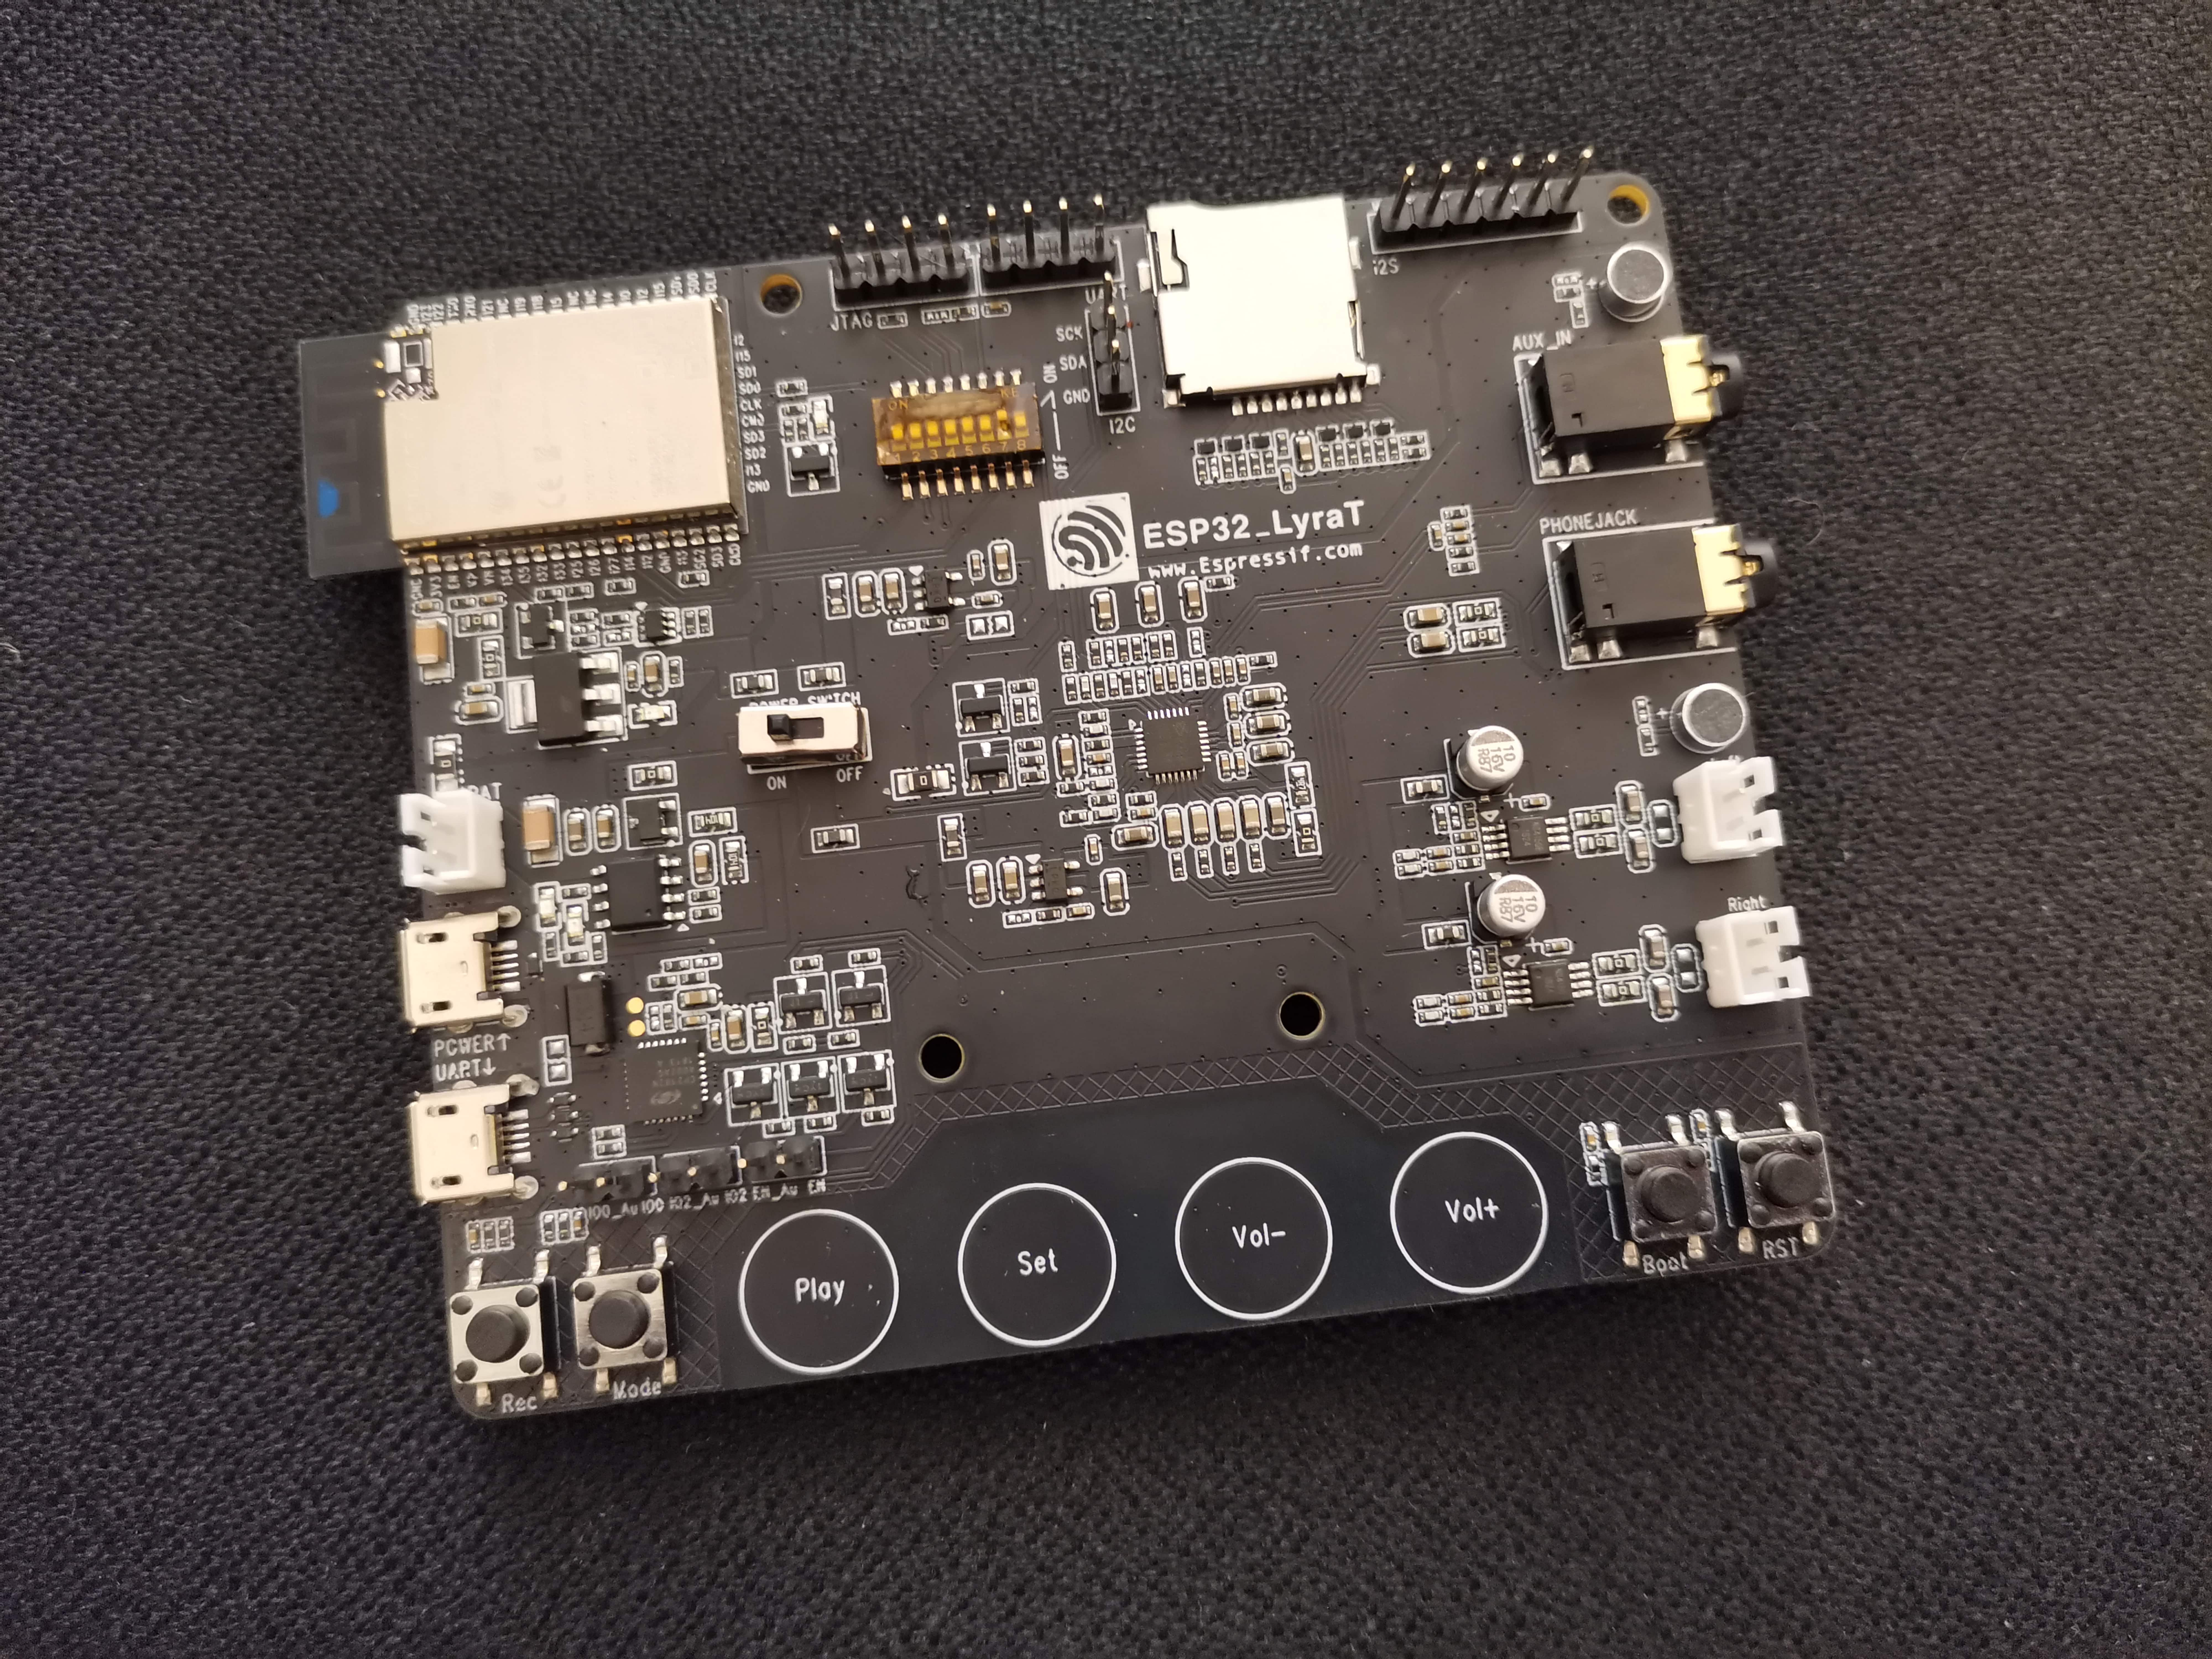
\includegraphics[width=1\linewidth]{images/ESP32-LyraT-1.jpg}
\end{minipage}%
\begin{minipage}{.5\textwidth}
  \centering
  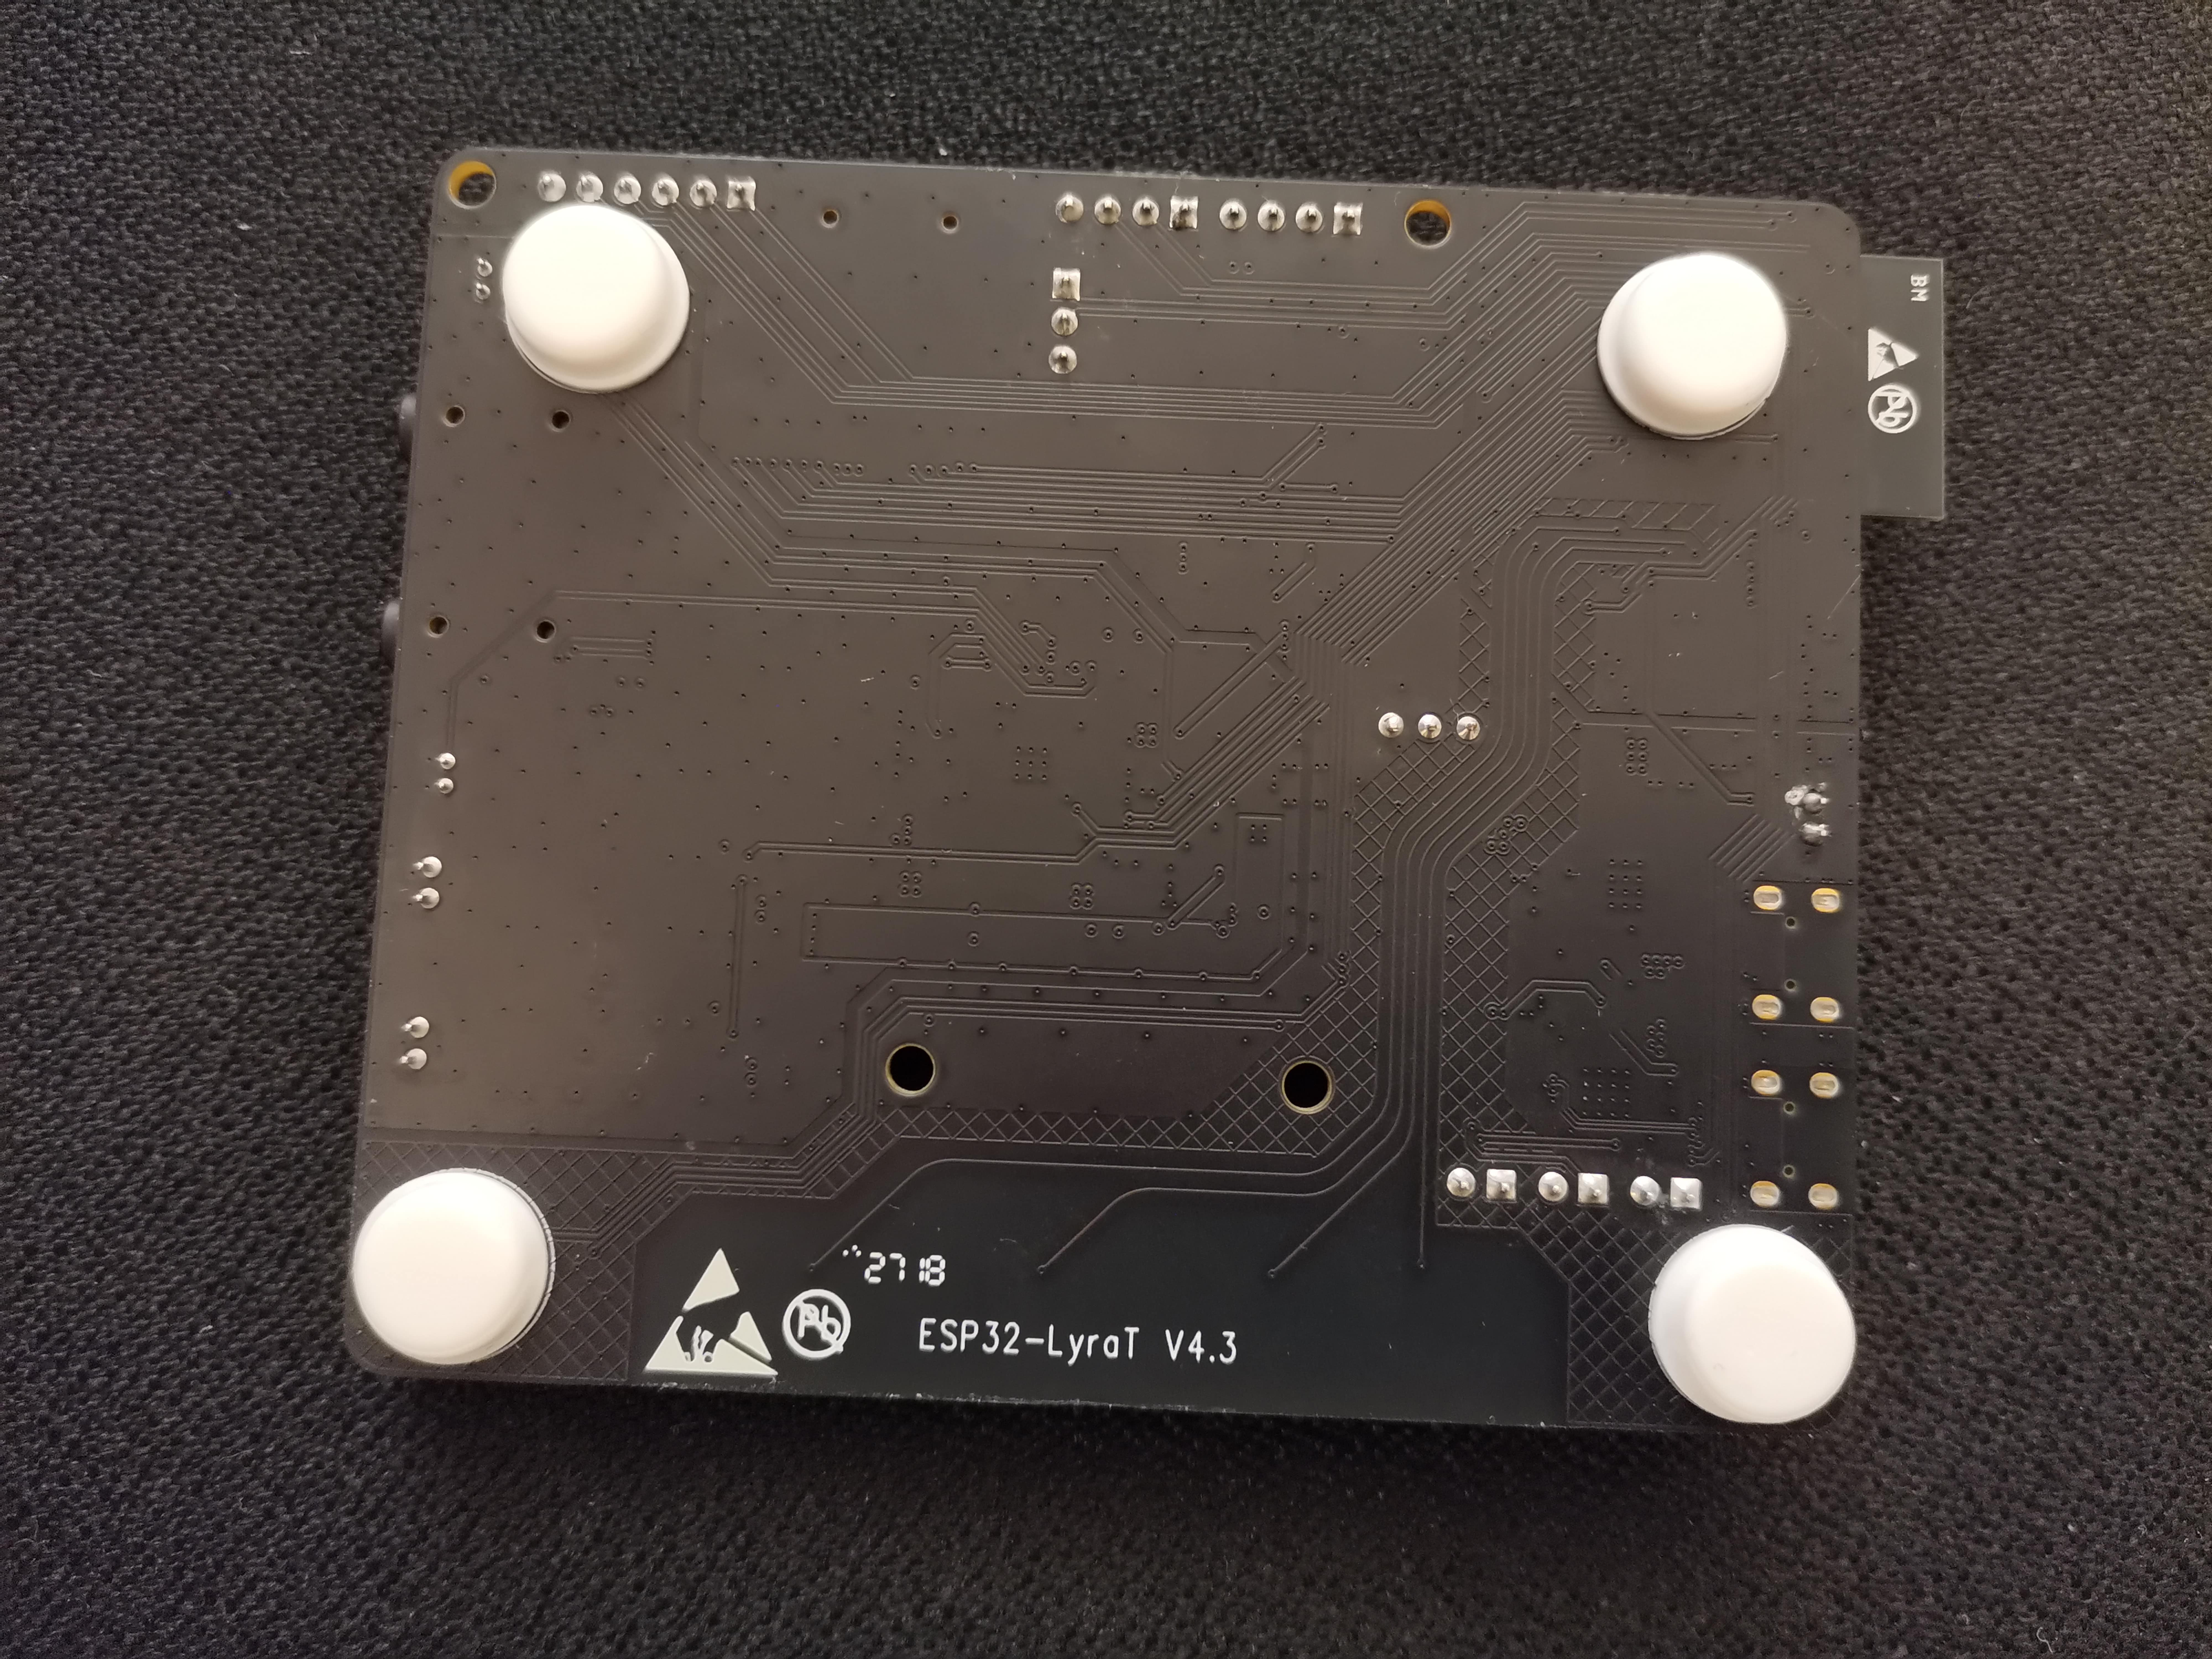
\includegraphics[width=1\linewidth]{images/ESP32-LyraT-2.jpg}
\end{minipage}
\caption{ESP32-LyraT}
\label{esp32-lyrat}
\end{figure}
\fi

\subsection{UOV}
Implementation can be found in folder \textit{src/esp/luov}. 

\subsection{Rainbow}
Implementation can be found in folder \textit{src/esp/rb}. 

%%%%%%%%%%%%%%%%%%%%%%%%%%%%%%%%%%%%%%%%%%%%
%%%%%%%%%%%%%%%%%%%%%%%%%%%%%%%%%%%%%%%%%%%%
\chapter{Testing and discussion}
\section{PC}
Security cathegories; graphs of times; memory from ref. pdf
\subsection{Time complexity}

%%%%%%%%%%%%%%%%%%%
\subsection{Memory complexity}

%%%%%%%%%%%%%%%%%%%%%%%%%%%%%%%%%%%%%%%%%%%%
\section{ESP32}
\subsection{Time complexity}
\begin{figure}[H]
\centering
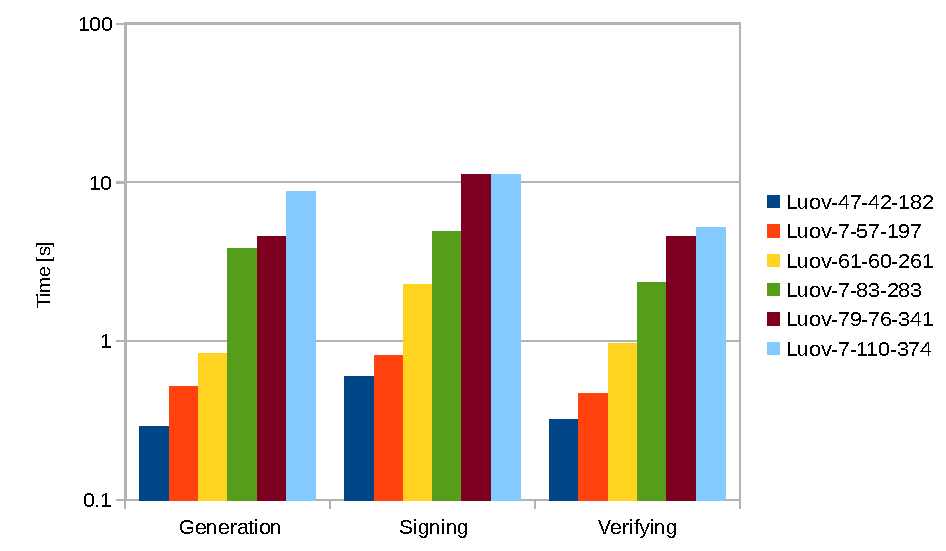
\includegraphics[width=13cm,height=7cm]{images/time-luov.pdf}
\caption{Porovnání naivních implementací}
\label{time-luov}
\end{figure}

\begin{figure}[H]
\centering
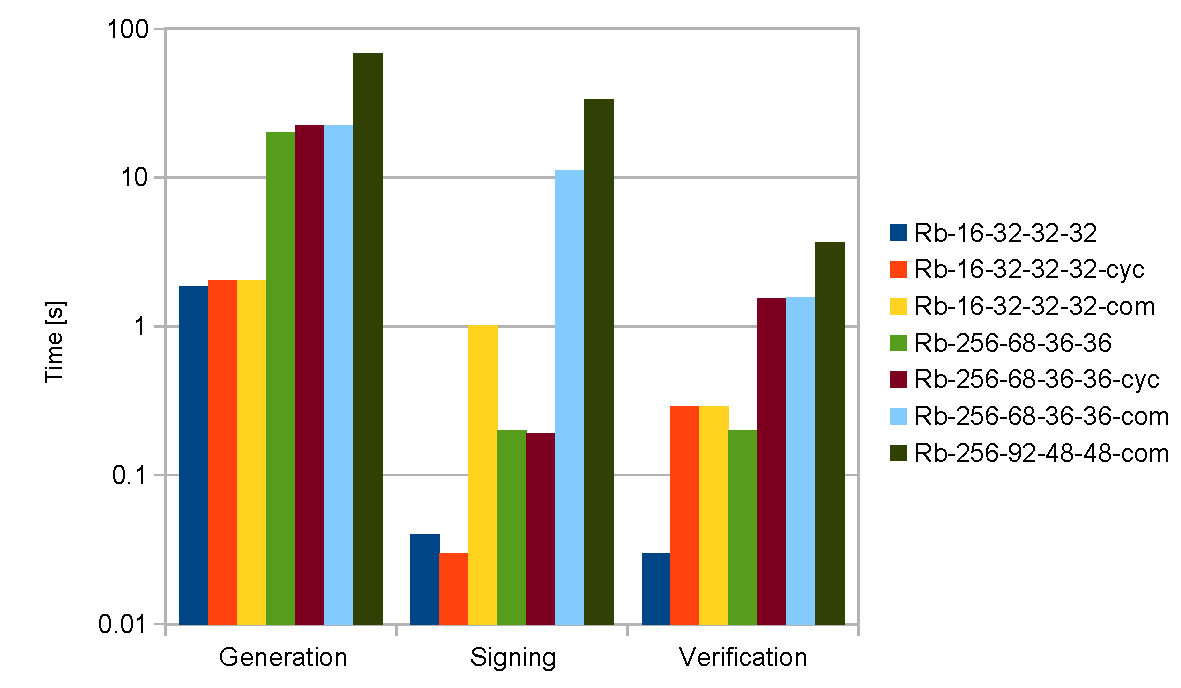
\includegraphics[width=13cm,height=7cm]{images/time-rb.pdf}
\caption{Porovnání naivních implementací}
\label{time-rb}
\end{figure}

\begin{figure}[H]
\centering
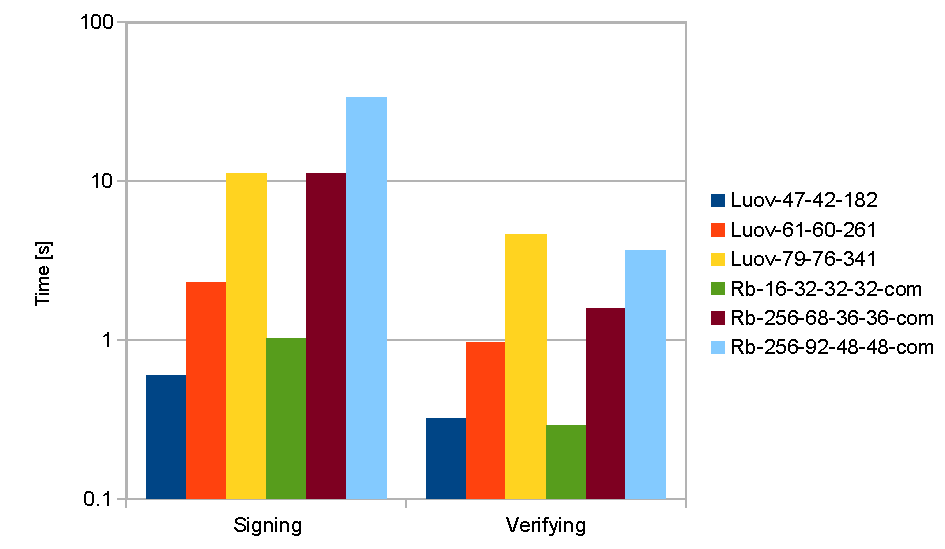
\includegraphics[width=13cm,height=7cm]{images/time-both.pdf}
\caption{Porovnání naivních implementací}
\label{time-both}
\end{figure}

%%%%%%%%%%%%%%%%%%%
\subsection{Memory complexity}
\begin{figure}[H]
\centering
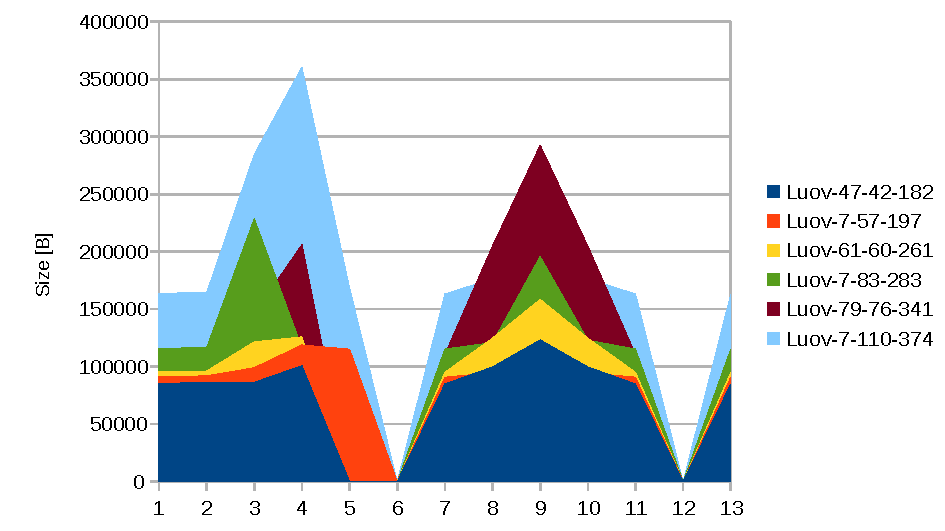
\includegraphics[width=13cm,height=7cm]{images/mem-luov0.pdf}
\caption{Porovnání naivních implementací}
\label{mem-luov0}
\end{figure}

\begin{figure}[H]
\centering
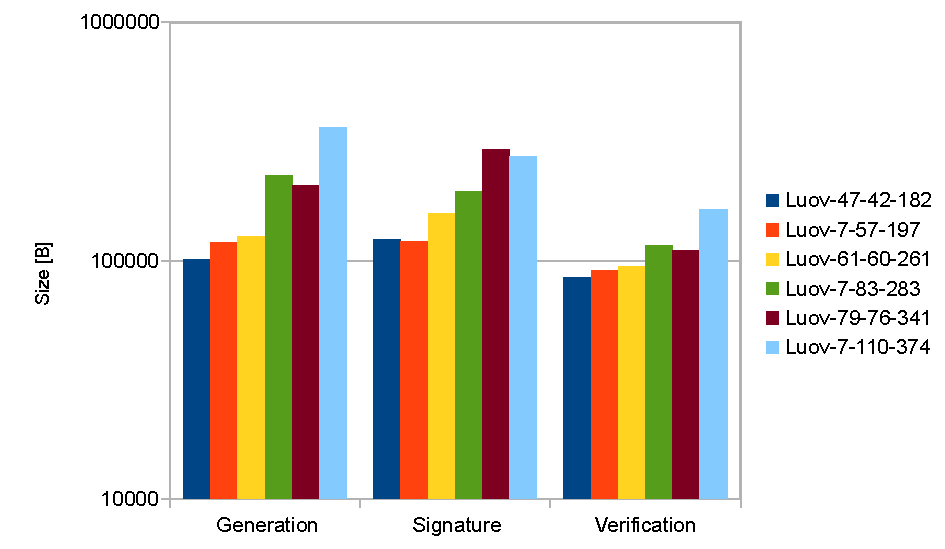
\includegraphics[width=13cm,height=7cm]{images/mem-luov.pdf}
\caption{Porovnání naivních implementací}
\label{mem-luov}
\end{figure}

\begin{figure}[H]
\centering
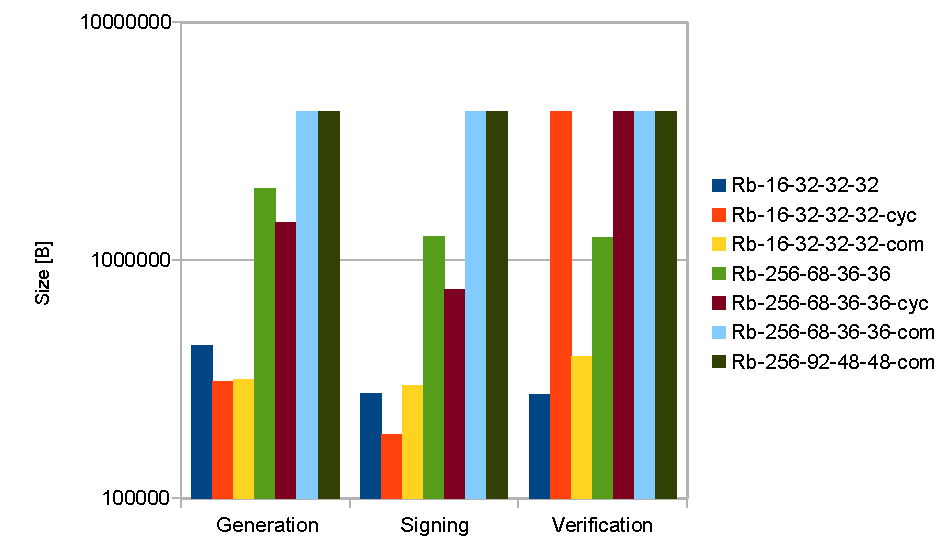
\includegraphics[width=13cm,height=7cm]{images/mem-rb.pdf}
\caption{Porovnání naivních implementací}
\label{mem-rb}
\end{figure}

\begin{figure}[H]
\centering
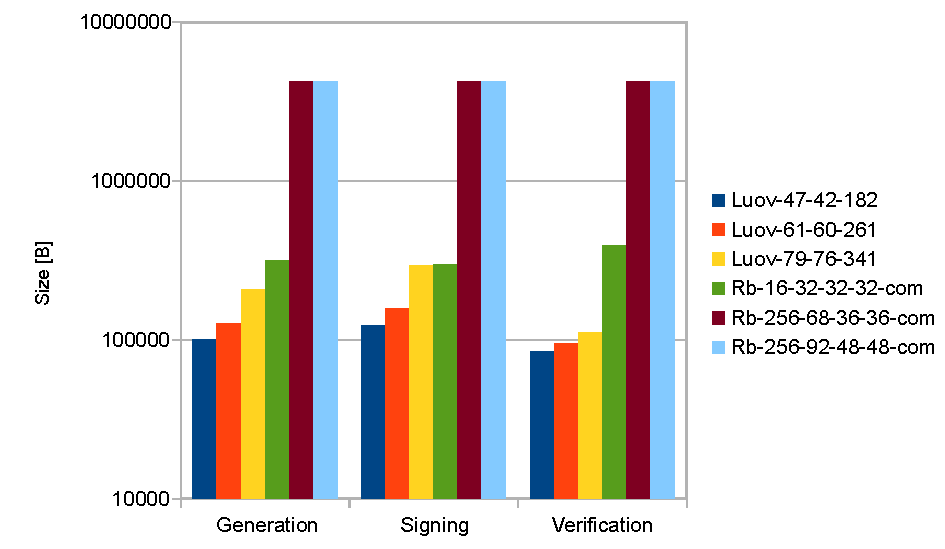
\includegraphics[width=13cm,height=7cm]{images/mem-both.pdf}
\caption{Porovnání naivních implementací}
\label{mem-both}
\end{figure}

\begin{figure}[H]
\centering
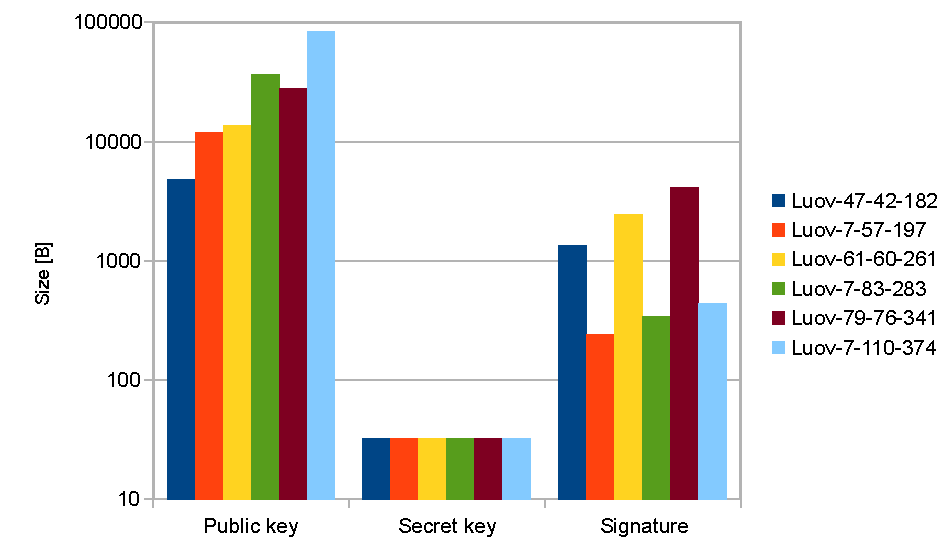
\includegraphics[width=13cm,height=7cm]{images/sign-luov.pdf}
\caption{Porovnání naivních implementací}
\label{sign-luov}
\end{figure}

\begin{figure}[H]
\centering
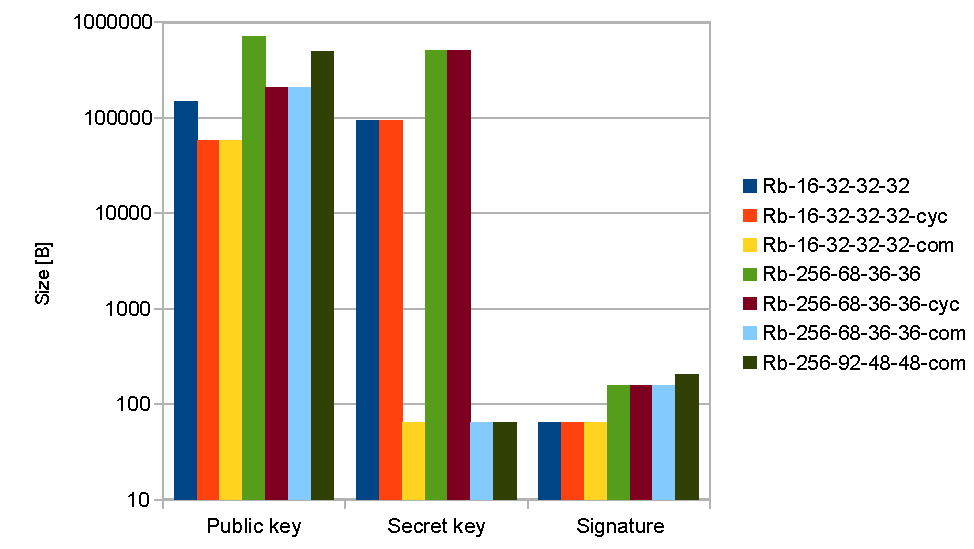
\includegraphics[width=13cm,height=7cm]{images/sign-rb.pdf}
\caption{Porovnání naivních implementací}
\label{sign-rb}
\end{figure}

%%%%%%%%%%%%%%%%%%%%%%%%%%%%%%%%%%%%%%%%%%%%
\section{Conventional algorithms}
RSA, ECDSA

\begin{figure}[H]
\centering
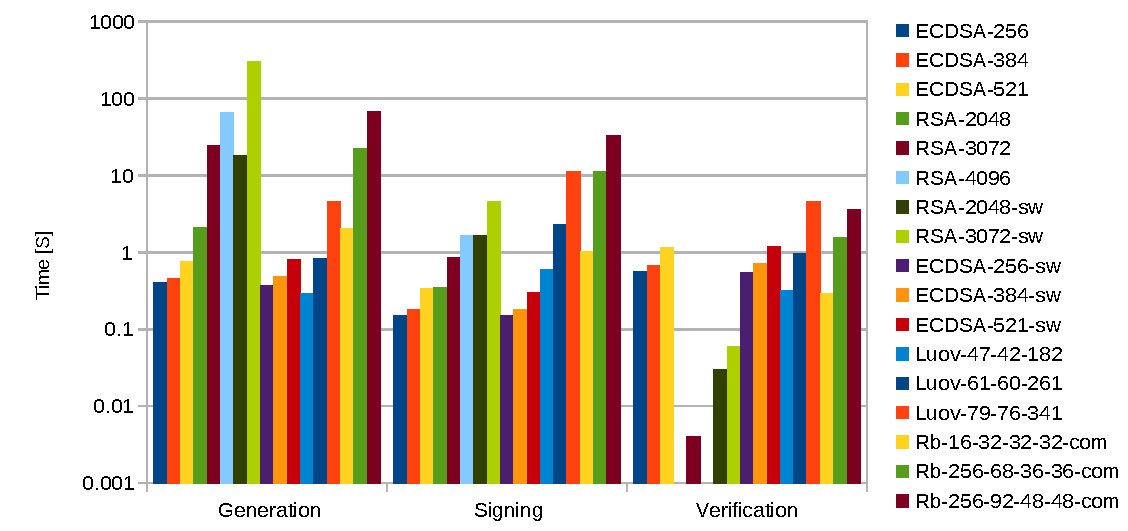
\includegraphics[width=13cm,height=7cm]{images/time-all.pdf}
\caption{Porovnání naivních implementací}
\label{time-all}
\end{figure}

\begin{figure}[H]
\centering
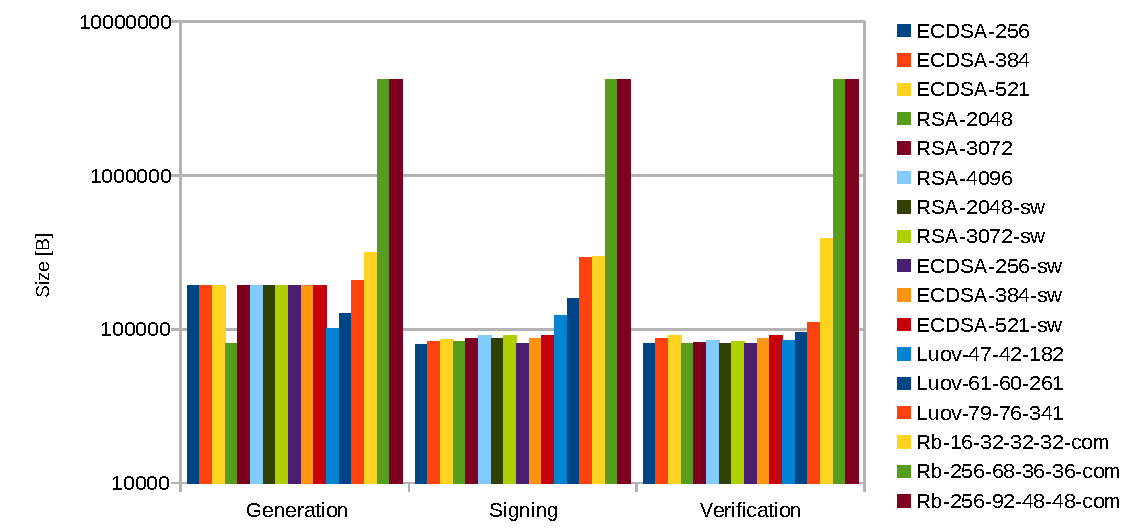
\includegraphics[width=13cm,height=7cm]{images/mem-all.pdf}
\caption{Porovnání naivních implementací}
\label{mem-all}
\end{figure}

%%%%%%%%%%%%%%%%%%%%%%%%%%%%%%%%%%%%%%%%%%%%
%%%%%%%%%%%%%%%%%%%%%%%%%%%%%%%%%%%%%%%%%%%%
\setsecnumdepth{part}
\chapter{Conclusion}
How good I was...; LOUV is much more better...

%%%%%%%%%%%%%%%%%%%%%%%%%%%%%%%%%%%%%%%%%%%%
%%%%%%%%%%%%%%%%%%%%%%%%%%%%%%%%%%%%%%%%%%%%
\bibliographystyle{iso690}
\bibliography{mybibliographyfile}

\begin{thebibliography}{9}
\bibitem{L-CZYP}
CZYPEK, P.: \textit{Implementing Multivariate Quadratic Public Key Signature Schemes on
Embedded Devices.}  Ruhr-Universit\"{a}t Bochum, 2012.

\bibitem{L-PET1}
PETZOLDT, A.: \textit{Multivariate Cryptography Part 1: Basics} [online]. 2017, [cit. 2020-04-1]. At: \url{https://2017.pqcrypto.org/school/slides/1-Basics.pdf}

\bibitem{L-PET2}
PETZOLDT, A.: \textit{Multivariate Cryptography Part 2: UOV and Rainbow} [online]. 2017, [cit. 2020-04-1]. At: \url{https://2017.pqcrypto.org/school/slides/2-UOV+Rainbow.pdf}

\bibitem{L-GEOV}
GEOVANDRO, C.C.F.P.: \textit{Introduction to Multivariate Public Key Cryptography} [online]. 2013, [cit. 2020-04-1]. At: \url{http://www.ic.unicamp.br/ascrypto2013/slides/ascrypto2013_geovandropereira.pdf}

\bibitem{L-MC0}
GOUBIN, L.; PATARIN, J.; YANG, BY.: \textit{Multivariate Cryptography.} In: van Tilborg H.C.A., Jajodia S. \textit{Encyclopedia of Cryptography and Security.} 2011, Springer, Boston, MA

\bibitem{L-MC1}
DING, J.; PETZOLDT, A.: \textit{Current State of Multivariate Cryptography.} In: \textit{IEEE Security \& Privacy.}, vol. 15, no. 4, pp. 28-36, 2017.

\bibitem{L-WIKI1}
\textit{Multivariate cryptography} [online]. 2020, [cit. 2020-04-1]. At: \url{https://en.wikipedia.org/wiki/Multivariate_cryptography}

\bibitem{L-KS98}
KIPNIS, A.; SHAMIR, A.: \textit{Cryptanalysis of the oil and vinegar signature scheme}. In \textit{CRYPTO 1998}, LNCS vol. 1462, pp. 257–266, Springer, 1998.

\bibitem{L-NIST-2ND}
\textit{NIST - Post-Quantum Cryptography, Round 2 Submissions} [online]. 2020, [cit. 2020-04-1]. At: \url{https://csrc.nist.gov/Projects/post-quantum-cryptography/round-2-submissions}

\bibitem{L-EQ-KEYS}
WOLF, CH.; PRENEEL, B.: \textit{Equivalent keys in multivariate quadratic public key systems}. In \textit{Journal of Mathematical Cryptology}, pp. 375–415, 2011.

\bibitem{L-LIFTING}
BEULLENS, W.; PRENEEL, B.: \textit{Field lifting for smaller UOV public keys}. In \textit{Progress
in Cryptology INDOCRYPT 2017: 18th International Conference on Cryptology in India}, Springer, 2017.

\bibitem{L-RB-CYC}
PETZOLDT, A.; BULYGIN, S.; BUCHMANN, J.: \textit{Multivariate
Signature Scheme with a Partially Cyclic Public Key.} In: \textit{INDOCRYPT.} 2010, vol. 6498, pp. 33 - 48. Springer, 2010.

\end{thebibliography}
%%%%%%%%%%%%%%%%%%%%%%%%%%%%%%%%%%%%%%%%%%%%
%%%%%%%%%%%%%%%%%%%%%%%%%%%%%%%%%%%%%%%%%%%%
\setsecnumdepth{all}
\appendix

\chapter{Acronyms}
% \printglossaries
\begin{description}
	\item[ECDSA] Elliptic Curve Digital Signature Algorithm
	\item[IoT] Internet of Things
	\item[LUOV] Lifted Unbalanced Oil and Vinegar
	\item[MC] Multivariate cryptography
	\item[MQ] Multivariate quadratics
	\item[NIST] National Institute of Standards and Technology
	\item[OV] Oil and Vinegar
	\item[PRNG] Pseudo-random number generator
	\item[UOV] Unbalanced Oil and Vinegar	
\end{description}


\chapter{Contents of enclosed CD}

%change appropriately

\begin{figure}
	\dirtree{%
		.1 readme.txt\DTcomment{the file with CD contents description}.
		.1 exe\DTcomment{the directory with executables}.
		.1 src\DTcomment{the directory of source codes}.
		.2 esp\DTcomment{implementation for esp32 platform}.
		.2 mathematica\DTcomment{implementation in Mathematica}.
		.2 offline\DTcomment{offline reference materials}.
		.2 esp\DTcomment{implementation for PC platform}.
		.2 thesis\DTcomment{the directory of \LaTeX{} source codes of the thesis}.
		.1 text\DTcomment{the thesis text directory}.
		.2 thesis.pdf\DTcomment{the thesis text in PDF format}.
	}
\end{figure}

\end{document}
